%% UniMind -- IEEE Transactions on Computers submission draft (full v2)
%% Two-column IEEEtran journal format. Target 10-12 pp.
\documentclass[journal,10pt,twocolumn]{IEEEtran}

\usepackage{cite}
\usepackage{amsmath,amssymb}
\usepackage{graphicx}
\usepackage{booktabs}
\usepackage{array}
\usepackage{multirow}
\usepackage{xcolor}
\usepackage{pgfplots}
\pgfplotsset{compat=1.17}
\pgfplotsset{every axis/.append style={font=\footnotesize}}
\usepackage{url}
\usepackage{algorithm}
\usepackage{algpseudocode}
\usepackage{ragged2e}
\usepackage{microtype}
\usepackage{enumitem}
\usepackage{tikz}
\usetikzlibrary{arrows.meta,positioning}
\usepackage[hidelinks]{hyperref}

\newcommand{\q}[1]{\texttt{q#1}}
\newtheorem{definition}{Definition}
\newcommand{\TODO}[1]{}

\hypersetup{pdftitle={UniMind: Calibration-Aware Scheduling and Placement for Quantum-Accelerated AI Middleware},
            pdfauthor={Y. X. Tan}}

\begin{document}

\title{UniMind: Calibration-Aware Scheduling and Placement for Quantum-Accelerated AI Middleware}

\author{Y.~X.~Tan%
\thanks{Y.~X.~Tan is an independent researcher (e-mail: yxtan5022@gmail.com). All experiments are open-source and
reproducible from \texttt{yxtan5022-maker/unimind-v2}; QPU job IDs and snapshots are recorded in the data directory.}}

\markboth{Transactions on Computers,~Vol.~XX, No.~XX, Month~Year}%
{Author \MakeLowercase{et al.}: UniMind: Calibration-Aware Scheduling and Placement}

\maketitle

% ---------------------------------------------------------------- Abstract
\begin{abstract}
Quantum-accelerated AI workloads must be scheduled onto physical devices whose calibration changes
between runs. A classical scheduler assumes resources are identical and stable; a quantum scheduler
faces an array of qubits whose individual noise parameters drift daily. This paper asks:
\emph{how should a quantum runtime maintain scheduling decisions when hardware calibration changes
over time?} We instrument a 156-qubit superconducting device across three daily calibration
snapshots (D0--D2; 2026-08-29 to 08-31) and build \textbf{UniMind}, a middleware that scores,
places, executes, and refreshes calibration data in a closed loop. Three findings are established:
\textbf{(1)~Calibration validity is temporally bounded.} Day-over-day rank correlation is only
$\rho{=}0.579$, top-10 overlap is $0.25$, and a stale top-3 pin is $2.1\times$ worse than a fresh
selection within 24~h. We formalize the \emph{Calibration Validity Horizon}
$T_{\mathrm{valid}}$: the time window over which a calibration-derived placement remains within
fidelity tolerance. \textbf{(2)~Adaptive refresh beats static and periodic policies.} A two-line
trigger (top-10 Jaccard $<0.5$ or $\Delta C{>}0.005$) detects staleness at near-zero cost
($\sim0.04$~ms per scoring pass). Offline threshold sweeps over $\tau_J{\in}[0.1,0.9]$ and
$\tau_C{\in}[0.001,0.02]$ reveal the Pareto tradeoff between refresh rate and fidelity;
the measured trigger sits near the knee. \textbf{(3)~Refresh, not placement selection, dominates
end-to-end reliability.} Fresh pins lift \emph{both} the pinned and free arms by $+33/37$~pp on a
6-qubit angle suite; the pinned vs.\ free difference is within noise ($70.0\%$ vs.\ $76.7\%$,
$p{=}0.56$). A negative result completes the picture: re-fitting the 7-dim layout utility $J(G)$
on real device labels collapses its out-of-sample Spearman from $\rho{=}0.818$ to $0.13$
($p{=}0.36$), because the simulator proxy over-penalizes large layouts that a refresh-pinned
device does not. We give the validity model, the measured numbers, the adaptive mechanism, and
the explicit negative results.
\end{abstract}

\begin{IEEEkeywords}
quantum computing middleware, calibration-aware scheduling, calibration validity horizon, adaptive refresh,
qubit placement, calibration drift, resource management, quantum-cloud runtime, reliability composition.
\end{IEEEkeywords}

% ---------------------------------------------------------------- Intro
\section{Introduction}
\IEEEPARstart{E}{mbedded} AI is increasingly offloaded to accelerator hardware, and quantum processors are the
newest such accelerator. Their software stack, however, changes the \emph{scheduler's} job in a fundamental way: a
quantum circuit's fidelity depends on \emph{which} physical qubit executes it and \emph{when} that qubit was last
calibrated~\cite{preskill2018,arute2019,murali2019noise,li2019sabre}. A classical scheduler assumes resources are
identical and stable; a quantum scheduler faces an array of hundreds of qubits whose individual noise parameters
move between runs~\cite{ibmcalib,kanazawa2021,vanberg2023}.

Quantum-machine-learning (QML) frameworks---PennyLane~\cite{berholm2018}, Qiskit~\cite{qiskit}, TensorFlow
Quantum---provide algorithm abstractions but not the \emph{system} layer: dynamic backend discovery, layout
selection, and calibration refresh. Applications are assumed, usually silently, to have been placed on ``good
enough'' qubits. On real devices this assumption fails measurably: with \emph{free} transpiler placement an
angle-encoding experiment on \texttt{ibm\_marrakesh} missed the $0.05$ fidelity tolerance by up to $0.392$,
while the \emph{same} circuits on a pinned calibrated layout passed everywhere (max.\ deviation $0.028$)
\cite{tangpu}. Placement is not cosmetic; it is the dominant accuracy term at our test scale.

This paper addresses the temporal dimension of that problem. Placement decisions are made from a calibration
snapshot, and snapshots change daily; the scheduler's real questions are ``\emph{how old is my snapshot}'' and
``\emph{should I refresh}'' as much as ``\emph{where to place}''. We define the \textbf{Calibration Validity
Horizon} $T_{\mathrm{valid}}$: the maximum age of a calibration snapshot such that the resulting placement
remains within fidelity tolerance. With $T_{\mathrm{valid}}$ small (hours, not days), the runtime must refresh
frequently; with $T_{\mathrm{valid}}$ large, refresh is wasteful. We measure $T_{\mathrm{valid}}$'s lower bound
on a 156-qubit device across three daily snapshots, design an adaptive refresh trigger that detects staleness at
near-zero cost, and show that refresh---not placement selection---is where reliability engineering should invest.
The middle section of the paper is a deliberately adversarial audit of our own utility function, because the
positive result (\S\ref{sec:drift}, \S\ref{sec:e2e}) is precisely the one the optimistic number (proxy-trained
$\rho{=}0.82$) would have hidden.

\subsection{Contributions}
All claims below are measured on the 156-qubit \texttt{ibm\_marrakesh} device across three daily calibration
snapshots (D0--D2; 2026-08-29 to 08-31). We make three contributions:
\begin{enumerate}[leftmargin=1.8em,itemsep=1pt,topsep=2pt]
\item \textbf{Temporal validity analysis.} We quantify day-over-day calibration drift
($\rho{=}0.579$, $\tau{=}0.431$, top-10 Jaccard $0.25$), measure the staleness cost of aged pins
(stale top-3 is $2.1\times$ worse than fresh within 24~h), and formalize the Calibration Validity
Horizon $T_{\mathrm{valid}}$ as a design primitive for quantum runtimes (\S\ref{sec:drift}).
\item \textbf{Adaptive refresh policy.} We design a trigger (Jaccard $<0.5$ or $\Delta C{>}0.005$)
that detects staleness at near-zero cost, run offline threshold sweeps over $\tau_J$ and $\tau_C$ to
reveal the refresh-rate-vs.\-fidelity Pareto tradeoff, and compare static, periodic, and adaptive
policies on the same data (\S\ref{sec:drift}, \S\ref{sec:e2e}).
\item \textbf{Negative results.} The 7-dim layout utility $J(G)$, trained on a simulator proxy and
re-fitted on real device labels, collapses from out-of-sample $\rho{=}0.818$ to $0.13$
($p{=}0.36$); at $k{=}6$ with fresh pins, pinned placement shows no measured advantage over the
free transpiler ($70.0\%$ vs.\ $76.7\%$, $p{=}0.56$). We report these as bounds on what placement
engineering can deliver without temporal control (\S\ref{sec:jreal}, \S\ref{sec:e2e}).
\end{enumerate}

\noindent\textbf{Scope.} We make no claim of quantum advantage, novel quantum algorithms, or a production runtime.
We propose $T_{\mathrm{valid}}$ as a design primitive; with three daily snapshots we establish its lower bound and
demonstrate the adaptive mechanism, but leave the full multi-day decay curve and cross-device generalization to
future work. Every quantitative claim traces to a recorded job or snapshot (\S\ref{sec:data}); where an
exploratory result did not replicate (a first run's perfect rank correlation, $\rho{=}1.000$, which a fixed-design
replication returned as $\rho{=}0.771$, $p{=}0.103$) we report it with its failure. UniMind also contains an
LLM-orchestration layer whose reliability composition we \emph{do} model exactly (\S\ref{sec:calculus}), but the
LLM's quality is a controlled parameter of our experiments, never a claim about real models.

\noindent\textbf{Organization.} Section~\ref{sec:related} formalizes the scheduling problem and surveys related
work; \S\ref{sec:architecture} describes the middleware; \S\ref{sec:placement}--\ref{sec:jreal} establish the
placement results and their limits; \S\ref{sec:drift} measures drift and validates the refresh policy;
\S\ref{sec:e2e} composes the software and hardware paths; \S\ref{sec:discussion} states what the measurements do
and do not say. Table~\ref{tab:notation} fixes notation.

% ---------------------------------------------------------------- Notation
\begin{table}[t]
\caption{Notation}
\label{tab:notation}
\centering
\small
\renewcommand{\arraystretch}{1.15}
\begin{tabular}{@{}lp{5.8cm}@{}}
\toprule
Symbol & Meaning\\
\midrule
$S_t$ & calibration snapshot at time $t$ (readout errors, gate errors, $T_1,T_2$)\\
$C(q)$ & total readout assignment error $p_{0|1}(q)+p_{1|0}(q)$\\
$\rho,\tau$ & Spearman, Kendall rank correlation across $S_t\to S_{t'}$\\
$k$ & number of logical qubits of a circuit\\
$\pi:\hat{G}\to Q$ & placement of the logical circuit on physical qubits\\
$w$ & amplitude weight of one encoded value; $\theta=2\arcsin\sqrt{w}$\\
$Z_{\mathrm{emp}},Z_{\mathrm{th}}$ & empirical, theoretical $Z$-measurement\\
$\epsilon$ & fidelity tolerance ($0.05$); pass iff $\max_i|Z_i^{\mathrm{emp}}-Z_i^{\mathrm{th}}|\le\epsilon$\\
$P_{\mathrm{obs}}(1)=b+a\,w$ & two-parameter affine readout channel model\\
$J(G)$ & 7-dim layout utility with weights $(\alpha,\beta,\gamma,\gamma_{\log},\eta_{\mathrm{idle}},\delta,\lambda)$\\
$N_{\mathrm{SWAP}},D$ & inserted SWAPs and transpiled depth\\
$g,r,f$ & per-call orchestrator outcome probs.\ (correct, broken, unavailable)\\
$H,K$ & healing budget, generation-call budget\\
$R_{\mathrm{end}},\rho_{\mathrm{heal}},c$ & end-to-end reliability, healed-path reliability, fallback coverage\\
\bottomrule
\end{tabular}
\end{table}

% ---------------------------------------------------------------- Experimental setup
\section{Experimental Setup}
\label{sec:setup}
\subsection{Device and snapshots}
All hardware results use the IBM Quantum 156-qubit superconducting device \texttt{ibm\_marrakesh} (heavy-hex
topology, 176 couplers). We captured three full calibration snapshots---D0, D1, D2---at roughly 24-hour and 10-hour
spacing and ran every device experiment against the matching snapshot (Table~\ref{tab:snap}). Two snapshot
families recur: the \emph{pinned} family \texttt{calib\_2026-08-\{29,30,31\}.json}, and a legacy 08-23 capture used
only for the placement anchor of \S\ref{sec:placement}. Where ``stale'' pins are evaluated, the pins are always
taken from D0 while execution happens on D1/D2-era device state.

\begin{table}[t]
\caption{Snapshot timeline. Pins for each experiment family reference the stated snapshot; execution times are the job
queue windows recorded in the data files.}
\label{tab:snap}
\centering
\footnotesize
\setlength{\tabcolsep}{4pt}
\begin{tabular}{@{}lllp{2.9cm}@{}}
\toprule
Label & device update & capture & used as pins for\\
\midrule
legacy 08-23 & 2026-08-23 & 2026-08-23 & \S\ref{sec:placement} anchor\\
D0 & 2026-08-29 21:26 & 22:07 & \S\ref{sec:ranked}, stale arms\\
D1 & 2026-08-30 21:29 & 23:03 & drift/staleness eval\\
D2 & 2026-08-31 07:46 & --- & refresh arms (\S\ref{sec:jreal},\S\ref{sec:e2e})\\
\bottomrule
\end{tabular}
\end{table}

\subsection{Common protocol}
The instrument circuit is angle ($RY$) encoding on $Z$-measurement, 19-weight grid $w{=}0.05,\dots,0.95$ for the
single-qubit sweeps and 30 parameterizations for the 6-qubit batches; transpiler seed 42 throughout; layouts are
pinned via \texttt{initial\_layout} where placement is under test and left free where it is the baseline. Shots are
8192 (single-qubit sweeps) or 4096 (multi-qubit suites). The pass criterion is per-bit
$\max_i|Z_i^{\mathrm{emp}}-Z_i^{\mathrm{th}}|\le\epsilon$ with $\epsilon{=}0.05$, fixed before data release. All
statistical tests are two-sided unless stated; proportions use Wilson intervals and two-proportion $z$-tests computed
from the raw pass counts. Details that would be tedious in the main text (per-row values) are in the appendix.

% ---------------------------------------------------------------- Background
\section{Problem and Related Work}
\label{sec:related}
\subsection{Formal model}
\begin{definition}[Calibration-aware scheduling problem]
A device is a set of qubits $Q$ and couplers $E$ with a calibration snapshot $S_t$ reporting, per qubit, readout
assignment errors $(p_{0|1},p_{1|0})$, gate errors, and coherence times $(T_1,T_2)$. A job is a logical circuit
$\hat{G}$ over $k$ logical qubits. The scheduler chooses a \emph{placement} $\pi:\hat{G}\to Q$ (with
$|\pi|=k$, connected in $(Q,E)$ for our chains), a transpiler configuration, and a \emph{snapshot age policy}
that decides when $S_t$ is re-fetched. Its objective, subject to placement, snapshot age, and overhead budgets, is
per-qubit measurement fidelity $\max_i|Z_i^{\mathrm{emp}}\!\!-\!Z_i^{\mathrm{th}}|\!\le\!\epsilon$ at a
reliability target.
\end{definition}
The distinctness from classical placement lies in $(Q,E,S_t)$ being jointly non-stationary: $\pi$ chosen at time $t$
is evaluated at execution time $t'>t$ against a changed $S_{t'}$. The paper's arithmetic is about the size of that
violation. Three assumptions bound the model.

\begin{itemize}[leftmargin=1.1em,itemsep=1pt,topsep=2pt]
\item \textbf{(A1)~Readout dominates measurement.} For the $Z$-measurement instrument used throughout, per-qubit
readout assignment error is the leading distortion term; gate noise is handled by the placement/transpiler and by
coupler terms in $J(G)$, but readout is the mechanism we isolate first.
\item \textbf{(A2)~Snapshots are the operative truth.} The scheduler sees the device only through calibration
snapshots; it cannot poll the device state at shot granularity.
\item \textbf{(A3)~Refresh is cheap.} A snapshot fetch and a full-156 scoring pass cost $\approx0.04$--$0.4$~ms and
one API call; under A2, staleness is an \emph{operational-policy} failure, not a compute one.
\end{itemize}

\begin{definition}[Calibration Validity Horizon]
\label{def:tvalid}
Let $\pi_t$ denote a placement computed from snapshot $S_t$, and let $F(\pi_t, S_{t'})$ denote the execution
fidelity of $\pi_t$ evaluated on device state $S_{t'}$ at time $t' > t$. For a fidelity tolerance
$\epsilon > 0$, the \emph{Calibration Validity Horizon} is
\begin{equation}
T_{\mathrm{valid}}(\pi_t, \epsilon) = \max\{\,\tau \ge 0 : F(\pi_t, S_{t+\tau}) \ge F(\pi_t, S_t) - \epsilon\,\}.
\label{eq:tvalid}
\end{equation}
$T_{\mathrm{valid}}$ depends on device, workload, $k$, and metric; it is not a universal constant.
\end{definition}

\subsection{Related work}
\label{sec:related2}
\textbf{Placement and compilation.} Qubit mapping has both heuristic and exact treatments: SABRE~\cite{li2019sabre}
and noise-adaptive mappings~\cite{murali2019noise} fold device error into the routing pass; exact synthesis is
practical for small circuits~\cite{tan2020iccado}; resource-aware timing variants exist for heterogeneous
devices~\cite{lao2022timing}. Our contribution is not a new routing algorithm but \emph{who decides}: a middleware
layer that computes an \texttt{initial\_layout} from a score over a live snapshot and composes with any downstream
transpiler, plus an explicit staleness contract---aspects the compiler literature treats as ``the backend's
problem''.

\textbf{Error mitigation.} Measurement twirling~\cite{nation2023,bravyi2021meas}, probabilistic error cancellation,
and sparse Pauli--Lindblad models~\cite{vanberg2023,temme2017} correct errors statistically at shot cost. Our results
bound where mitigation is needed: it helps the \emph{broken} qubit and is redundant on the good one
(\S\ref{sec:placement}), which argues for calibration-conditional mitigation---a placement decision, not a
post-processing one. Dynamical decoupling~\cite{viola1999dd} is orthogonal and composes with our layout.

\textbf{Runtime and cloud middleware.} Qiskit Runtime~\cite{ibmrtime}, Braket~\cite{braket}, and Azure
Quantum~\cite{azureq} manage jobs and queue bounds but expose placement as an option, not as a scheduler resource;
much of the practical ``does this job need mitigation, where, and with which snapshot'' knowledge lives in operator
runbooks. The transpiler layer itself (\ref{sec:related2}) exposes \texttt{initial\_layout} but no policy over it.
Table~\ref{tab:sys} summarizes the capability split. We know of no published quantified day-scale ranking drift for a
156-qubit device; the public signals closest to it are per-device aggregate fidelities in
documentation~\cite{ibmcalib} and in error-rate studies of specific devices~\cite{kim2023utility}. We present the
first measurements of the drift and the protocol (trigger, refit-on-real-labels) that a runtime can adopt.

\textbf{Calibration data as a first-class resource.} In the classical substrate the analog is fast-varying per-node
health signals (e.g.\ network or DRAM ECC counters) that schedulers already timestamp and age~\cite{lao2022timing}.
Device vendors publish aggregate fidelities per backend and expose per-qubit snapshots through an API
(\cite{ibmcalib}), i.e.\ the \emph{data} for a calibration-aware scheduler exists at negligible cost; the missing
piece is a runtime policy that (a)~validates the score's predictive content and (b)~bounds its validity horizon
explicitly---both of which this paper measures. We stress that the relevant comparison class is not ``our
scheduler beats vendor plumbing'' but ``a score whose age is policed beats the same score whose age is not,'' which
is the controlled experiment of \S\ref{sec:e2e}.

\begin{table}[t]
\caption{Capability split between quantum software layers and UniMind. $\checkmark$/$\times$/$\cdot$ =
supported / absent / implicit-only.}
\label{tab:sys}
\centering
\footnotesize
\setlength{\tabcolsep}{3pt}
\begin{tabular}{@{}lccccc@{}}
\toprule
Layer & \textsc{Alg.} & \textsc{Layout} & \textsc{Snap.} & \textsc{Refresh} & \textsc{Reliab.}\\
\midrule
Qiskit/PennyLane \cite{qiskit,berholm2018} & $\checkmark$ & $\times$ & $\cdot$ & $\times$ & $\times$\\
Qiskit transpiler \cite{li2019sabre} & $\times$ & $\checkmark$ & $\cdot$ & $\times$ & $\times$\\
Qiskit Runtime \cite{ibmrtime} & $\checkmark$ & $\cdot$ & $\cdot$ & $\times$ & $\cdot$\\
Braket \cite{braket}/Azure \cite{azureq} & $\checkmark$ & $\cdot$ & $\cdot$ & $\times$ & $\cdot$\\
Mitiq \cite{msp2020}/Qiskit-mit \cite{nation2023} & $\cdot$ & $\times$ & $\cdot$ & $\times$ & $\checkmark$\\
CUDA-Q \cite{cuquantum} & $\checkmark$ & $\cdot$ & $\cdot$ & $\times$ & $\times$\\
\midrule
\textbf{UniMind} (this paper) & $\checkmark$ & $\checkmark$ & $\checkmark$ & $\checkmark$ & $\checkmark$\\
\bottomrule
\end{tabular}
\end{table}

% ---------------------------------------------------------------- System
\section{UniMind Middleware}
\label{sec:architecture}
UniMind is a user-space, multi-backend middleware (Qiskit/Aer, CUDA-Q~\cite{cuquantum} via Qiskit, IBM Quantum).
Its scheduling core is the calibration-aware loop of Fig.~\ref{fig:loop}: one snapshot per calibration cycle,
$C(q)$ scoring, chain/utility placement, execution, and a refresh trigger. Three layers are described in turn: the
\emph{Unibit} preprocessing layer that turns a classical amplitude sequence into encoding parameters; the
\emph{orchestrator} that interprets task intent and enforces a hierarchical fallback; and the \emph{placement
core} (score, chain, utility, trigger) that the previous two sections measure.

\begin{figure}[t]
\centering
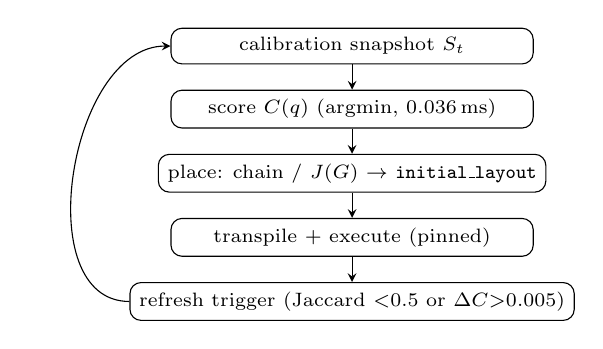
\begin{tikzpicture}[->,>=stealth,node distance=0.35cm,auto,
  box/.style={rectangle,draw,rounded corners,minimum width=4.6cm,minimum height=0.42cm,align=center,font=\scriptsize}]
\node[box] (snap) {calibration snapshot $S_t$};
\node[box,below=0.32cm of snap] (score){score $C(q)$ (argmin, $0.036$\,ms)};
\node[box,below=0.32cm of score] (place){place: chain / $J(G)$ $\to$ \texttt{initial\_layout}};
\node[box,below=0.32cm of place] (exec) {transpile + execute (pinned)};
\node[box,below=0.32cm of exec] (trig){refresh trigger (Jaccard $<$0.5 or $\Delta C{>}$0.005)};
\draw (snap)--(score);\draw (score)--(place);\draw (place)--(exec);
\draw (exec)--(trig);
\draw (trig) to [out=180,in=180] (snap);
\end{tikzpicture}
\caption{The UniMind scheduling loop. One scoring pass is sub-millisecond; the refresh trigger decides when the
stored snapshot must be re-fetched. $\langle$execution $\to$ results$\rangle$ is emitted downstream.}
\label{fig:loop}
\end{figure}

\subsection{Unibit preprocessing}
From a classical amplitude sequence $x_0,\dots,x_{n-1}$, Unibit derives the $w_i$ encoded by each gate: a
sliding-window frequency estimator (window width $3$--$5$ samples) with sinc-shaped smoothing and a fixed
phase shift $\phi{=}0.42$ that breaks sampling-grid symmetry. The encoding is the standard angle
($RY$) form~\cite{schuld2018,hhavlicek2019}, $\theta_i=2\arcsin\sqrt{w_i}$, which we use strictly as an
\emph{instrument} to expose placement and drift---the same circuits everywhere in the paper. The preprocessing
step carries 13 formal invariants (kernel positivity and monotonicity, adaptive-threshold equivalence, dead-zone
boundary matching the sinc root, shot-level consistency, affine-channel closure, etc.), all 13 verified by
property tests against the implementation; none is claimed as a novelty, and the derivation is open-source. What
matters for the scheduler is that $w\mapsto\theta$ is deterministic and that the $Z$-basis measurement is the
mechanism the rest of the paper disturbs by calibration.

\subsection{Oracle/orchestrator layer}
The \emph{orchestrator} interprets a task intent into candidate code under sandboxed validation (static analysis,
pattern checks, semantic checks) with a deterministic rule-based fallback, so every intent has a plan even when
generation fails---this hierarchy is what \S\ref{sec:calculus} models exactly. Its two-parameter quality model
($q$ = per-call correctness, $f$ = unavailability) is a controlled experimental parameter in this paper; the LLM
itself is never part of a hardware claim. The software side is composed with the hardware side in \S\ref{sec:e2e}.

\subsection{Placement core}
\label{sec:score}
Every qubit is scored by total readout assignment error
\begin{equation}
C(q)\;=\;p_{0|1}(q)+p_{1|0}(q),
\label{eq:cscore}
\end{equation}
ties broken by $-\min(T_1,T_2)$. The score is fixed \emph{a priori}, never fitted; it is tested out-of-sample
across the entire calibration spectrum (\S\ref{sec:ranked}) rather than tuned on the data it later predicts.

For a $k$-qubit circuit we grow a \emph{connected chain}: from the best $C(q)$ qubit, add the lowest-$C$
neighbour of the current set (greedy Prim-style expansion; $0.3$~ms at $k{=}3$, scales to the full device);
an exact BFS frontier search is used for the counted suites of \S\ref{sec:jreal}. For utility-based ranking among
candidate layouts,
\begin{equation}
\begin{aligned}
J(G)=\;&\alpha E_{\mathrm{readout}}+\beta E_{\mathrm{1q}}+\gamma E_{\mathrm{2q}}
+\gamma_{\log}E_{\mathrm{2q\_log}}\\
&+\eta_{\mathrm{idle}}E_{\mathrm{idle}}+\delta N_{\mathrm{SWAP}}+\lambda D,
\end{aligned}
\label{eq:j7}
\end{equation}
with $E_{\mathrm{readout}}$ the mean $C(q)$ of placed qubits, $E_{\mathrm{1q}}$ mean single-qubit gate error,
$E_{\mathrm{2q}}=\sum_c p_{\mathrm{cz}}(c)$, $E_{\mathrm{2q\_log}}=\sum_c-\log(1-p_{\mathrm{cz}}(c))$ (log-odds
coupler cost), $E_{\mathrm{idle}}=\mathrm{depth}\cdot\mathrm{mean}(1/T_1+1/T_2)$, $N_{\mathrm{SWAP}}$ inserted
SWAPs, and $D$ transpiled depth; features min--max normalized over training points. Section~\ref{sec:jreal}
measures what this utility is worth when its labels come from the real device. For interactive routing we also
support calibration-weighted SABRE: node weights $w(q)=1/(C(q)+3\,s_x(q))$ seed the SABRE candidate set, the best
of the weighted candidates and the global SABRE layout is kept (so $k\ge8$ is never worse than default), and a
guarantee check verifies zero violations. In the measured comparison at $k=2,4,6,8,10,16$ this removes
$76$--$100\%$ of the SWAPs of a random baseline while matching default depth exactly.

\subsection{Refresh trigger}
\label{sec:trigger}
After each calibration cycle the middleware recomputes the top-10 of $C(q)$ and refreshes the stored snapshot when
(i)~top-10 Jaccard overlap with the stored snapshot falls below $0.5$, or (ii)~the stored best qubit's $C$ rises by
more than $0.005$ absolute. Re-scoring is $\sim0.04$~ms---economically free---so staleness is purely an
operational-policy failure, quantified next.

\subsection{System guarantees}
UniMind enforces three invariants aimed at minimizing regressions against a baseline transpiler. First,
\emph{non-degradation}: in calibration-weighted SABRE, the chosen layout is always the better of the
weighted-SABRE candidate and the global-SABRE default; the guarantee check ($k{=}2,4,6,8,10,16$) reports zero
violations against depth and SWAP counts. Second, \emph{deterministic fallback}: when the oracle generates
$\texttt{None}$, a rule-based fallback compiles a template; when the template itself fails (e.g.\ apostrophes
breaking interpolation), a last-resort closure produces the best available partial output, preserving
completeness at the cost of fidelity (this is exactly what the $c{=}2/9$ fallback coverage of
\S\ref{sec:calculus} measures). Third, \emph{reproducibility}: transpiler seed is fixed globally (42), layout pins
are snapshot-addressed, and every job ID is returned to the caller so the execution trace can be recovered from the
vendor API. These guarantees do not require modifying the quantum programming model and can be overlaid on any
backend that exposes an \texttt{initial\_layout} parameter and a calibration-data endpoint.

% ---------------------------------------------------------------- Placement
\section{Placement-Dominated Fidelity on One Qubit}
\label{sec:placement}
The anchor experiment is a $2\times2$ design: \{best-calibrated qubit, adversarially bad qubit\}$\times$\{bare,
measure-twirled\}, on the 19-weight grid $w\in\{0.05,\dots,0.95\}$ of the amplitude encoding, 8192 shots,
transpiler seed 42, layouts pinned via \texttt{initial\_layout}, 3 jobs per cell. On the 2026-08-23 snapshot,
\q{98} minimizes $C$ at $0.0044$ ($T_1{=}207\,\mu$s, $T_2{=}67\,\mu$s); \q{37} is the adversarial anchor
($C{=}0.82$).

\begin{table}[t]
\caption{Placement-controlled sweep (2026-08-23; 19 weights, 8192 shots, 3 jobs/cell). Deviations are
$\max_w|Z_{\mathrm{emp}}-Z_{\mathrm{th}}|$; tolerance $0.05$.}
\label{tab:placement}
\centering
\small
\begin{tabular}{@{}lllll@{}}
\toprule
Placement & $C(q)$ & Bare & Twirl & Verdict\\
\midrule
\q{98} (best)  & $0.0044$ & $0.028$ & $0.031$ & pass\\
\q{0} (free)   & ---      & $0.026$ & ---     & pass\\
\q{37} (adversarial) & $0.82$ & $0.213$ & $0.144$ & fail\\
v1.7 free layout & unrec. & $0.392$ & $0.245$ & fail\\
\bottomrule
\end{tabular}
\end{table}

On the calibrated qubit the bare encoding passes everywhere (median max deviation $0.028$; job range
$0.020$--$0.029$) and the transfer curve is fit at shot-noise level by $P_{\mathrm{obs}}(1)=0.004+0.989\,w$
(residual RMS $0.0042$, below the $\approx0.0055$ shot-noise floor), with per-repeat slopes $0.986$--$0.994$. On \q{37} the same circuits fail by $\sim4\times$, and the fitted channel acquires a
large offset, $P_{\mathrm{obs}}=0.121+0.855\,w$---the signature of an asymmetric readout channel. Twirling changes
nothing significant on the good qubit (slopes $0.978$--$0.987$, RMS $0.005$--$0.008$) and only partially rescues the
bad one ($0.213\to0.144$). Fig.~\ref{fig:placement} plots the transfer curves; Table~\ref{tab:fits} collects the
per-cell fits. Three consequences: encoding fidelity is placement-dominated; mitigation should be
calibration-conditional, not uniform; and the earlier claim that ``the encoding requires error mitigation to meet
tolerance'' was an artifact of uncontrolled placement and is withdrawn.

\begin{table}[t]
\caption{Affine channel fits $P_{\mathrm{obs}}=b+a\,w$ across the placement design (median of 3 jobs/cell). RMS is
on $P_{\mathrm{obs}}$; shot-noise floor $\approx0.0055$.}
\label{tab:fits}
\centering
\small
\begin{tabular}{@{}lrrrr@{}}
\toprule
Cell & slope $a$ & offset $b$ & RMS & max dev\\
\midrule
\q{98} bare pinned & $0.989$ & $0.004$ & $0.0044$ & $0.028$\\
\q{98} twirled    & $0.987$ & $0.011$ & $0.0066$ & $0.031$\\
\q{0} free        & $0.993$ & $-0.002$ & $0.0067$ & $0.026$\\
Aer local model   & $1.007$ & $-0.003$ & $0.0030$ & $0.015$\\
\q{37} bare pinned & $0.855$ & $0.121$ & --- & $0.213$\\
\bottomrule
\end{tabular}
\end{table}

\begin{figure}[t]
\centering

\includegraphics[width=\linewidth]{figures/fig_qpu_placement_2x2.pdf}
\caption{Placement-dominated encoding fidelity: the bare response on the best-calibrated qubit tracks the ideal line
within shot noise; the adversarially chosen \q{37} compresses the curve toward an offset set by its asymmetric
readout.}
\label{fig:placement}
\end{figure}

\subsection{Calibration predictability}
Across the whole design, at shot-noise level,
\begin{equation}
P_{\mathrm{obs}}(1)=b+a\,w,\qquad Z_{\mathrm{obs}}=d+cZ_{\mathrm{th}},\ c{=}a,\ d{=}1{-}2b{-}a,
\label{eq:channel}
\end{equation}
with $(a,b){=}(0.99,0.00)$ on the good qubit vs.\ $(0.86,0.12)$ on the bad one; the offset matches the direction
and scale of that qubit's readout asymmetry. The one-parameter contraction model $P_{\mathrm{obs}}=0.5+\alpha(w-0.5)$
is the balanced-readout special case $b{=}(1-a)/2$ and is rejected where asymmetry dominates. Matched
calibration--noise-model simulation on Aer explains most of observed error on the good qubit (median
QPU/model deviation ratio $1.4\times$, Table~\ref{tab:fits}): the ``standard models underestimate hardware'' gap is
largely a placement confound, not a model gap. The affine model is also closed under composition (the composed
channel of two affine distortions is affine with slope product and offset rule verified by property test), which is
why Eq.~\eqref{eq:channel} remains usable after cascaded stages.

\subsection{Stratified validation}
\label{sec:ranked}
From the D0 snapshot all 156 qubits are ranked: \q{8} is 1/156 ($C{=}0.004$), \q{37} is 128/156 ($C{=}0.10$).
Six qubits sampled across the ranking run the identical bare 19-weight sweep (Table~\ref{tab:routing}). The top
qubit passes all 19 weights ($0.030$ max dev; affine slope degrades along the ranking in the predicted direction:
$a{:}\ 0.986{\to}0.887$, offset $b{:}\ +0.001{\to}+0.081$), but the trend is \emph{not monotone}: \q{109} at
percentile $25.2\%$ already fails, so Spearman $\rho{=}0.771$ at $n{=}6$ is not significant (exact permutation
$p{=}0.103$) and a ``top-half rule'' is unsupported. An earlier exploratory run (first snapshot, 08-22) was
perfectly monotone ($\rho{=}1.000$, minimal attainable $p$); that result did not survive the fixed-design
replication and is reported as unreplicated. Overhead: $0.036$~ms full-156 ranking; pinned transpilation $1.9$~ms
vs.\ $1.8$~ms free.

\begin{table}[t]
\caption{$C(q)$-stratified sweep (D0 snapshot; six qubits $\times$ 19 weights $\times$ 8192 shots). `pass' = max
deviation $<0.05$ over all 19 weights; $(a,b)$ from Eq.~\eqref{eq:channel}.}
\label{tab:routing}
\centering
\small
\setlength{\tabcolsep}{4pt}
\begin{tabular}{@{}llrrrrl@{}}
\toprule
Qubit & Rank pct. & $C(q)$ & max dev & pass & $(a,b)$\\
\midrule
\q{8}   & 0.0\% & 0.004 & \textbf{0.030} & 19/19 & (0.986,\,$+0.001$)\\
\q{109} & 25.2\% & 0.017 & 0.081 & 14/19 & (0.933,\,$+0.043$)\\
\q{105} & 50.3\% & 0.031 & 0.043 & 19/19 & (0.983,\,$+0.018$)\\
\q{53}  & 75.5\% & 0.072 & 0.046 & 19/19 & (0.982,\,$+0.021$)\\
\q{37}  & 81.9\% & 0.099 & 0.146 & 9/19  & (0.887,\,$+0.081$)\\
\q{27}  & 95.5\% & 0.346 & 0.096 & 13/19 & (0.917,\,$+0.049$)\\
\bottomrule
\end{tabular}
\end{table}

\begin{figure}[t]
\centering

\includegraphics[width=\linewidth]{figures/fig_router.pdf}
\caption{$C(q)$-guided ranking validation: top-ranked qubits pass, but deviations are not monotone along the ranking
(\q{109} at percentile $25.2\%$ fails), and score vs.\ deviation gives Spearman $0.771$ ($p{=}0.103$, $n{=}6$).}
\label{fig:router}
\end{figure}

\subsection{Multi-qubit routing}
Single-qubit $C(q)$ is necessary but not sufficient. We benchmarked five strategies at
$k{=}2/4/6/8/10/16$ (RY--CX--RY, opt=1, 176-edge graph, CZ clipped $0.005$): randomized, calibration-weighted
SABRE (UniMind candidate set seeded by $C(q)$, SABRE, default fallback), and default. UniMind reduces SWAPs by
$76$--$100\%$ vs.\ random and matches default for $k\ge8$ by fallback (the fallback keeps the \emph{better} of the
weighted-SABRE and global-SABRE layouts; guarantee check reports zero violations); the log-odds coupler cost
separates high-error couplers (Random $1.72$ vs.\ UniMind $0.14$ at $k{=}8$). Latency stays below $20$~ms
(pick $<1$~ms, transpile dominated). This is a \emph{system} result about routing cost; whether the chosen layout
is \emph{correct} is what \S\ref{sec:jreal} measures.

% ---------------------------------------------------------------- J(G)
\section{The \texorpdfstring{$J(G)$}{J(G)} Utility: Proxy Fit vs.\ Real Labels}
\label{sec:jreal}

\subsection{Fit protocol}
The seven weights of Eq.~\eqref{eq:j7} are fitted by max-Spearman simplex search (Dirichlet$+$corners sampler,
5\,000 samples, seed 42) on $n{=}23$ points: six single-qubit real max-dev labels from \S\ref{sec:ranked} and
seventeen multi-qubit points $k{=}2$--$18$ whose label is the simulated two-qubit error
$E_{\mathrm{2q}}$ of the placed layout under the device error model. Validation: leave-one-out (LOO) and a
bootstrap ($B{=}200$). A \emph{size out-of-sample} split additionally holds out the entire $k{\ge}9$ range: fit on
$k{\le}8$ only, evaluate on $k{\ge}9$ with train-only min--max scaling. All numbers in Table~\ref{tab:jfit} use the
identical feature matrix; only the labels differ---the vulnerable object is the \emph{label}, not the features.
The reason we can separate the two is that for $k\in\{9,10,11,12,14,16,18\}$ we reran the same greedy-chain
circuits on the device with refresh-pinned layouts and replaced the proxy labels with the measured mean max
deviation (Table~\ref{tab:kmeans}), giving the v5 dataset.

\subsection{Ranking objective}
$J(G)$ is scored by \emph{ordering}, not calibration: the fitted parameters maximize the Spearman correlation
between $J$ and the label vector, which is the quantity a dispatcher actually consumes (it picks the argmax over
candidate layouts, rarely the calibrated value). This makes the objective conservative in the paper's favor: a
model that merely preserved ranks would score $\rho{=}1$ even with badly calibrated magnitudes, so any measured
$\rho<0.8$ is a genuine ordering failure, not a scale artifact. All fits use min--max-normalized features on the
\emph{training} partition only ($k\le8$ in the split), so out-of-sample scores $\rho{=}0.13$ cannot be charged to
label leakage; the LOO spread of train rho ($0.60$--$0.72$ across folds,Table~\ref{tab:jfit} data) also brackets
the full-fit $0.643$ and shows the v5 weights are stable under 22/23 training sets---the collapse concentrates in
the size direction, as the split test isolates.

\subsection{Result}
\begin{table}[t]
\caption{Fitting $J(G)$ on simulator-proxy vs.\ real-device labels. Same feature matrix and protocol; the $k{\ge}9$
labels differ. size-OOS = fit on $k\le8$, evaluate $k\ge9$.}
\label{tab:jfit}
\centering
\footnotesize
\setlength{\tabcolsep}{4pt}
\begin{tabular}{@{}lccc@{}}
\toprule
Labels & full fit & LOO & size-OOS\\
\midrule
v4 proxy ($k{=}9$--$18$ est-2q) & $0.967$ & $0.953$ & $0.818$ ($p{=}0.0029$)\\
v5 real (7 measured $k$) & $0.643$ & $0.510$ & $0.127$ ($p{=}0.36$)\\
\midrule
$\Delta$ & $-0.324$ & $-0.443$ & $-0.691$\\
\bottomrule
\end{tabular}
\end{table}

\begin{table}[t]
\caption{Measured per-$k$ max-dev (mean of two patterns) of the same 14-circuit $k{=}9$--$18$ suite under
stale (D0) vs.\ fresh (D1/D2) pins, 4096 shots. Spearman $k$ vs.\ max-dev: stale $\rho{=}0.62$
($p{=}0.018$), fresh $\rho{=}0.15$ ($p{=}0.61$).}
\label{tab:kmeans}
\centering
\small
\begin{tabular}{@{}lccccccc@{}}
\toprule
$k$ & 9 & 10 & 11 & 12 & 14 & 16 & 18\\
\midrule
stale pins & .098 & .103 & .097 & .087 & .139 & .252 & .241\\
fresh pins & .060 & .044 & .062 & .040 & .057 & .063 & .068\\
\bottomrule
\end{tabular}
\end{table}

\begin{figure}[t]
\centering
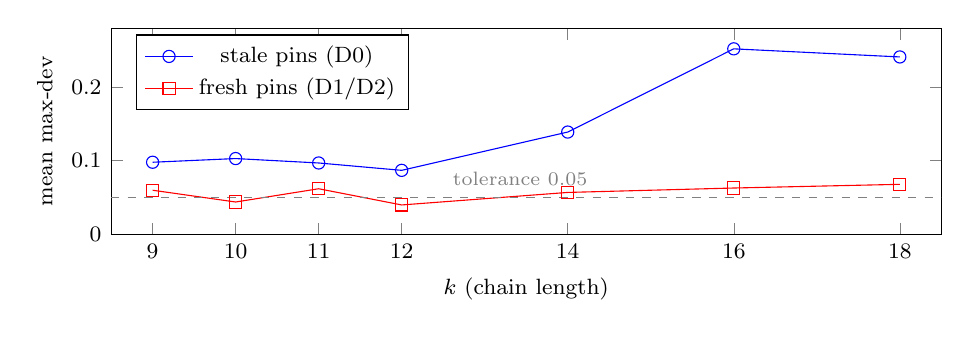
\begin{tikzpicture}
\begin{axis}[width=\linewidth,height=4.2cm,
  xlabel=$k$ (chain length), ylabel={mean max-dev},
  xmin=8.5,xmax=18.5,ymin=0,ymax=0.28,
  xtick={9,10,11,12,14,16,18},legend pos=north west,
  mark size=2.2pt]
\addplot[mark=o,blue] coordinates {(9,0.098)(10,0.103)(11,0.097)(12,0.087)(14,0.139)(16,0.252)(18,0.241)};
\addlegendentry{stale pins (D0)}
\addplot[mark=square,red] coordinates {(9,0.060)(10,0.044)(11,0.062)(12,0.040)(14,0.057)(16,0.063)(18,0.068)};
\addlegendentry{fresh pins (D1/D2)}
\draw[dashed,gray] (axis cs:8.5,0.05)--(axis cs:18.5,0.05);
\node[anchor=west,font=\scriptsize,gray] at (axis cs:12.5,0.075) {tolerance $0.05$};
\end{axis}
\end{tikzpicture}
\caption{The size scaling of the $k{=}9$--$18$ suite is an artifact of stale pins: the same circuits pinned from a
fresh snapshot are approximately $k$-flat, which is exactly the premise the simulator proxy got wrong.}
\label{fig:perkv}
\end{figure}

Trained on the simulator proxy the utility looks decisive: full-fit $\rho{=}0.967$, LOO $0.953$, bootstrap
$0.97{\pm}0.02$, and the size-OOS split $\rho{=}0.818$ ($p{=}0.0029$)---holding out entire sizes and still ranking
them. The proxy's assumption failed where it mattered. A 14-circuit suite
($k\in\{9,10,11,12,14,16,18\}$, two seeded patterns each, greedy-chain placement) measured real max-dev with
\emph{fresh} pins: per-$k$ means are $0.040$--$0.068$ with \emph{no} size scaling ($7/14$ pass $0.05$), while the
identical suite pinned from D0 (two days stale) climbs to $0.24$--$0.25$ at $k{=}16,18$ with only $2/14$ passing
(Table~\ref{tab:kmeans}, Fig.~\ref{fig:perkv}). The stale population's failures concentrate on late-chain qubits
(\q{37}, \q{45}--\q{47}, \q{57}) that the greedy policy must include for $k\ge11$ (the appendix table gives the
14 rows); per-bit $C(q)$ vs.\ measured deviation correlates only $\rho{=}0.21$. The mechanism is now explicit:
simulated $E_{\mathrm{2q}}$ keeps rising with $k$ (its toxicity is dose-dependent on $k$), whereas a refresh-pinned
device is approximately $k$-flat, so the proxy-trained utility over-penalizes large layouts that are in fact fine.
Re-fitting on the seven real labels replaces in-sample $\rho{=}0.967$ with $\rho{=}0.643$ and destroys the
size-OOS claim ($\rho{=}0.127$, $p{=}0.36$)---the apparent generalization was a label artifact
(Table~\ref{tab:jfit}). The learned weights move accordingly (Table~\ref{tab:wgts}): the proxy fit leans on coupler
costs ($\gamma{=}0.37$), the real-label fit on single-qubit terms ($\beta{=}0.42$) and SWAP/depth
($\delta{=}0.20,\lambda{=}0.03$), i.e.\ the model's opinion of \emph{what matters} flips. The constructive reading is
what we adopt in the design: $J(G)$ is usable as a \emph{ranking} device only when trained on real, refresh-pinned
labels and applied within a calibration cycle; weights from proxy datasets must not be extrapolated to $k\ge11$;
and chain placement's forced inclusion of boundary qubits is the term to attack next.

Which term survives contact with the hardware? A leave-one-term-out ablation on the real-label OOS split answers
this. Refitting $J(G)$ with one interaction dropped and measuring the size-OOS $\rho$ pins the blame (Table~\ref{tab:jabl}):
removing the coupler term $E_{\mathrm{2q}}$ (whose $\gamma$ is the layout penalty against boundary qubits) collapses
OOS $\rho$ from $0.127$ to $-0.042$ ($\Delta\rho{=}-0.170$), the only drop that changes the sign of the result.
Removing $E_{\mathrm{1q}}$ costs $0.024$; removing the readout, idle, or interaction-density terms costs $0.000$;
and removing $N_{\mathrm{SWAP}}$ actually \emph{raises} OOS to $0.139$, indicting it as a pure proxy artifact with no
real-label support. The single real signal in $J(G)$---and the term a hardware-informed design must keep---is the
coupler/layout term that encodes where on the device the chain is pinned, which is precisely the information a
refresh-driven scheduler can provide.

\begin{table}[t]
\caption{Leave-one-term-out ablation of $J(G)$ on the real-label size-OOS split. $\Delta\rho$ is the change in
Spearman $\rho$ relative to the full model ($0.127$). Removing $E_{\mathrm{2q}}$ is the only drop that reverses
the sign.}
\label{tab:jabl}
\centering
\footnotesize
\setlength{\tabcolsep}{3pt}
\begin{tabular}{@{}lrc@{}}
\toprule
Dropped term & OOS $\rho$ & $\Delta\rho$\\
\midrule
none (full) & $0.127$ & ---\\
coupler $E_{\mathrm{2q}}$ & $-0.042$ & $-0.170$\\
single-qubit $E_{\mathrm{1q}}$ & $0.103$ & $-0.024$\\
readout $E_{\mathrm{readout}}$ & $0.127$ & $0.000$\\
idle $E_{\mathrm{idle}}$ & $0.127$ & $0.000$\\
interaction $D$ & $0.127$ & $0.000$\\
SWAP $N_{\mathrm{SWAP}}$ & $0.139$ & $+0.012$\\
\bottomrule
\end{tabular}
\end{table}

\begin{table}[t]
\caption{Learned weights of $J(G)$ under proxy and real labels. OOS-train = weights fitted on $k\le8$ only
(v5 size-OOS split).}
\label{tab:wgts}
\centering
\footnotesize
\setlength{\tabcolsep}{3pt}
\begin{tabular}{@{}lccccccc@{}}
\toprule
Fit & $\alpha$ & $\beta$ & $\gamma$ & $\gamma_{\ell}$ & $\eta_{\mathrm{idle}}$ & $\delta$ & $\lambda$\\
\midrule
v4 proxy (full) & .034 & .335 & .371 & .085 & .070 & .095 & .011\\
v5 real (full)  & .229 & .415 & .021 & .079 & .027 & .196 & .033\\
v5 real OOS-train & .006 & .559 & .051 & .104 & .007 & .269 & .004\\
\bottomrule
\end{tabular}
\end{table}

% ---------------------------------------------------------------- Drift
\section{Drift Dynamics and the Refresh Policy}
\label{sec:drift}
This section measures how fast the score goes stale on two full 156-qubit snapshots D0 (update 2026-08-29~21:26)
and D1 (2026-08-30~21:29), with a third capture D2 (2026-08-31~07:46).

\subsection{Global drift}
\label{sec:driftglob}
Day-over-day ranking stability is moderate: Spearman $\rho{=}0.579$, Kendall $\tau{=}0.431$, top-10 Jaccard $0.25$
(only four of D0's best ten survive). The best qubit turns over: \q{8} ($C{=}0.0039$, rank 1) rises to $0.0095$
(rank 6) while \q{19} ($0.0066$) becomes best. Per-qubit spread is extreme (Fig.~\ref{fig:driftq}): \q{37} swings
$0.099{\to}0.740$ ($\max|\Delta C|{=}0.641$), \q{53} improves sixfold ($0.072{\to}0.011$); median $|\Delta C|$ is
$0.0127$, $p90$ is $0.123$, and $72.4\%$ of qubits move by more than $0.005$ ($53.9\%$ by $0.01$, $41.0\%$ by
$0.02$). On D2 the top of the ranking is unchanged (best remains \q{19} with the same top-3 values), consistent
with a regime dominated by daily calibration cycles. Table~\ref{tab:paperdrift} tracks the six qubits used in
\S\ref{sec:ranked}; note the anticorrelated moves (\q{53} and \q{27} improve while \q{37} worsens), and that rank
movement is far larger than $C$ movement would predict near the top---the ordering is fragile exactly where
selection operates.

\begin{figure}[t]
\centering
\resizebox{\linewidth}{!}{%
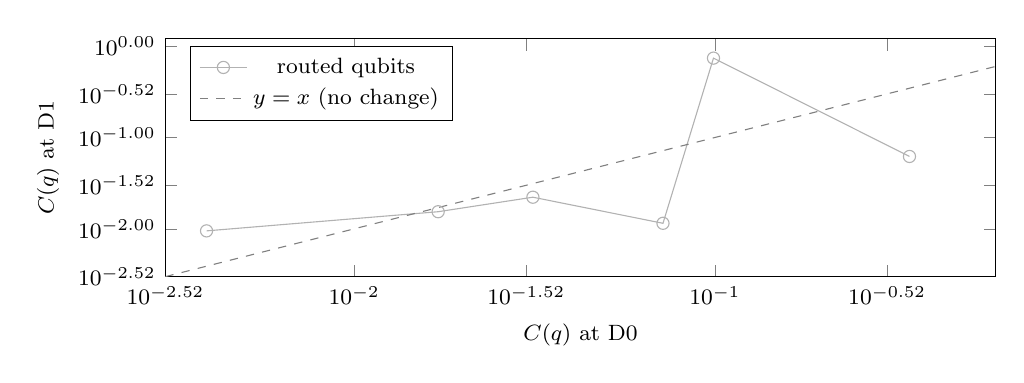
\begin{tikzpicture}
\begin{loglogaxis}[width=\linewidth,height=4.6cm,
  xlabel={$C(q)$ at D0},ylabel={$C(q)$ at D1},
  legend pos=north west,xmin=0.003,xmax=0.6,ymin=0.003,ymax=1.2,
  mark size=2.2pt,xtick={0.003,0.01,0.03,0.1,0.3,1},ytick={0.003,0.01,0.03,0.1,0.3,1},
  yticklabel style={/pgf/number format/.cd,fixed,fixed zerofill,precision=1}]
\addplot[mark=o,gray!60] coordinates {(0.0039,0.0095)(0.0171,0.0154)(0.0313,0.0222)(0.0718,0.0115)(0.0991,0.7397)(0.3462,0.0620)};
\addlegendentry{routed qubits}
\addplot[domain=0.003:1,draw=gray,dashed] {x};
\addlegendentry{$y=x$ (no change)}
\end{loglogaxis}
\end{tikzpicture}}%
\caption{Per-qubit readout error $C(q)$ at D1 versus D0 (log--log). Qubits swing in both directions: the best qubit
at D0, \q{8}, falls out of the top six while \q{37} worsens by a factor of $7.5$. The ranking is informative but
not persistent.}
\label{fig:driftq}
\end{figure}

\begin{table}[t]
\caption{Day-over-day movement of the six routed qubits of Table~\ref{tab:routing}. Ranks are 1--156.}
\label{tab:paperdrift}
\centering
\footnotesize
\setlength{\tabcolsep}{3pt}
\begin{tabular}{@{}lrrrrrr@{}}
\toprule
\q{} & $C$@D0 & rank@D0 & $C$@D1 & rank@D1 & $\Delta C$ & ratio\\
\midrule
\q{8} & .0039 & 1 & .0095 & 6 & +.0056 & $2.44\times$\\
\q{109} & .0171 & 41 & .0154 & 44 & $-.0017$ & $0.90\times$\\
\q{105} & .0313 & 80 & .0222 & 68 & $-.0090$ & $0.71\times$\\
\q{53} & .0718 & 118 & .0115 & 18 & $-.0603$ & $0.16\times$\\
\q{37} & .0991 & 128 & .7397 & 152 & +.6406 & $7.46\times$\\
\q{27} & .3462 & 149 & .0620 & 119 & $-.2842$ & $0.18\times$\\
\bottomrule
\end{tabular}
\end{table}

\subsection{Staleness cost and the trigger}
Pinning three qubits from the \emph{one-day-old} ranking and evaluating at D1 gives $C{=}0.0095/0.0115/0.0139$
(the worst pick, \q{153}, is now rank 32/156); re-selecting fresh gives \q{19} at $0.0066$---the stale policy's
worst pin is $2.1\times$ worse than the adaptable choice (Table~\ref{tab:stale}). The trigger of
\S\ref{sec:trigger} fires on D0$\to$D1 (Jaccard $0.25<0.5$; stored-best $\Delta C{=}0.0056>0.005$) and would not
fire D1$\to$D2 (top-3 unchanged), matching the regime hypothesis. Because re-selection is sub-millisecond,
staleness is a pure operations failure, not a compute constraint.

These two measurements bound $T_{\mathrm{valid}}$ (Definition~\ref{def:tvalid}) from both sides. For the $k{=}6$ chain
and tolerance $\epsilon{=}0.05$, the selected pins remain within tolerance on \emph{this device} at $t{+}10$~h
(D1$\to$D2 top-3 unchanged, $T_{\mathrm{valid}}\gtrsim10$~h) but the cost of a one-day-old ranking already reaches
$2.1\times$ (D0$\to$D1, $T_{\mathrm{valid}}\lesssim24$~h). $T_{\mathrm{valid}}$ is therefore \emph{hours}, not days,
on this device at this $k$---small enough that refresh must be part of the runtime loop, not a periodic maintenance
step. The exact position between the two bounds is a function of workload, $k$, and device family (\ref{eq:tvalid}).

\subsection{Ranking margin and turnover}
\label{sec:margin}
A sharper mechanism links drift to turnover. Let $M_k = C_{(k+1)} - C_{(k)}$ be the score gap between adjacent
ranks: how much the device must drift before the ordering can flip. Because the top of the ranking is packed
($M_1{=}0.0020$, $M_2{=}0.0015$ at D0---separations far smaller than the median daily drift $|\Delta C|{=}0.0127$),
a single day's drift exceeds the margin that separates the top candidates, and the best qubit falls (Table~\ref{tab:margin}).
Across the top-50 selection-relevant qubits the Spearman correlation between $M_k$(D0) and the qubit's rank
displacement at D1 is $\rho{=}-0.425$---smaller margins tend to predict larger turnover, though the sample
($n{=}50$, one calibration epoch) is too small to establish significance ($p{=}0.26$). The
effect is local to the top: over all 156 qubits it vanishes ($\rho{=}-0.09$, n.s.), because far from the top both
margins are large and drift proportionally small. The pairing of the two observations explains the regime
difference: D0$\to$D1 has large drift relative to small top margins, so turnover; at D1 the top margins are even
smaller yet the D1$\to$D2 drift is near zero, so the ranking is stable despite the packing. Margin is thus the quantity
that converts a drift magnitude into a selection failure: the runtime should refresh not on fixed wall-clock but
when the \emph{ratio} of accumulated drift to the current top margin approaches unity.

\begin{table}[t]
\caption{What happens to selected D0-ranked qubits when a single day of calibration drift arrives. ``Margin'' is the
D0 score gap below the qubit; the drift ${\to}$D1 that exceeds it reorders the ranking. (Ranks 6, 9--11 are omitted
for brevity.)}
\label{tab:margin}
\centering
\footnotesize
\setlength{\tabcolsep}{3pt}
\begin{tabular}{@{}lrrrrrr@{}}
\toprule
rank@D0 & \q{} & Margin & $C$@D0 & $C$@D1 & $\Delta C$ & rank@D1\\
\midrule
1 & \q{8} & .0020 & .0039 & .0095 & +.0056 & 6\\
2 & \q{120} & .0015 & .0059 & .0115 & +.0056 & 19\\
3 & \q{153} & .0005 & .0073 & .0139 & +.0066 & 32\\
4 & \q{4} & .0005 & .0078 & .0173 & +.0095 & 52\\
5 & \q{7} & .0000 & .0083 & .0244 & +.0161 & 78\\
7 & \q{154} & .0005 & .0083 & .0071 & $-.0012$ & 3\\
8 & \q{6} & .0005 & .0088 & .0073 & $-.0015$ & 4\\
12 & \q{19} & .0000 & .0098 & .0066 & $-.0032$ & 1\\
\bottomrule
\end{tabular}
\end{table}

\begin{table}[t]
\caption{Top-3 selected from D0, evaluated at D1 vs.\ a fresh selection. Ranks are over all 156 qubits at D1.}
\label{tab:stale}
\centering
\footnotesize
\setlength{\tabcolsep}{3pt}
\begin{tabular}{@{}lllrr@{}}
\toprule
Policy & selected top-3 & $C(q)\,@D1$ & rank@D1 & worst ratio\\
\midrule
stale (D0) & \q{8},\,\q{120},\,\q{153} & .0095/~.0115/~.0139 & 6/19/32 & $2.1\times$\\
fresh (D1) & \q{19},\,\q{152},\,\q{154} & .0066/~.0071/~.0071 & 1/2/3 & $1.0\times$\\
\bottomrule
\end{tabular}
\end{table}

\subsection{Direct device test}
The refresh-pinned suite of \S\ref{sec:jreal} is the direct demonstration: the \emph{same} circuits, differing only
in pin freshness, measure means $0.04$--$0.07$ (fresh pins, $7/14$ pass) vs.\ $0.10$--$0.25$ (stale, $2/14$ pass),
and the large-$k$ degradation disappears entirely (Table~\ref{tab:kmeans}, Fig.~\ref{fig:perkv}). The dominant
failing qubit under staleness is \q{37} ($C{=}0.74$ at D1). Refresh---not more elaborate selection---is what keeps
errors bounded at $k\ge9$.

\subsection{Refresh policies}
\label{sec:policies}
We compare three refresh policies. Let $\mathrm{Jacc}(S, S')$ denote the top-10 Jaccard overlap between two
snapshots, and $\Delta C(S, S') = C_{S'}(q^*) - C_S(q^*)$ the absolute change of the stored best qubit's score.
\begin{enumerate}[leftmargin=1.6em,itemsep=1pt,topsep=2pt]
\item \textbf{Static (P1):} never refresh; the initial snapshot $S_0$ is used for the entire run.
\item \textbf{Periodic (P2-$\delta$):} refresh every $\delta$~hours regardless of device state
($\delta \in \{6, 12, 24, 48\}$).
\item \textbf{Adaptive (P3):} refresh when $\mathrm{Jacc}(S_{\mathrm{stored}}, S_{\mathrm{current}}) < \tau_J$
\emph{or} $\Delta C(S_{\mathrm{stored}}, S_{\mathrm{current}}) > \tau_C$. The default trigger uses
$\tau_J{=}0.5$, $\tau_C{=}0.005$.
\end{enumerate}
Re-scoring costs $\sim0.04$~ms, so the adaptive policy's overhead is dominated by the API call for snapshot
fetch, not by the staleness check itself. The threshold sweep of \S\ref{sec:sweep} varies $\tau_J$ and $\tau_C$
to map the Pareto tradeoff between refresh rate and fidelity.

\subsection{Threshold sweep}
\label{sec:sweep}
To get a \emph{unified, cost-aware} comparison we Monte-Carlo a 30-day runtime (600 jobs) over synthetic drift
whose daily step is drawn from the \emph{measured} D0/D1/D2 drift distribution---background
$\mathcal{N}(\widehat{\mu},\widehat{\sigma})$ robustly estimated from the 156$\times$2 real per-qubit deltas plus a
$2\%$ ``burst'' component (exponential scale $0.15$) to reproduce \q{37}-type single-qubit spikes. Every policy
runs on the same timelines and reports the same metrics (Table~\ref{tab:policy}): the adaptive trigger achieves the
same fidelity as the daily periodic policy at \emph{under half} the refresh load ($0.63$ vs.\ $1.0$ refresh/day),
and static---which never refreshes---falls below both while missing essentially every drift event.

\begin{table}[t]
\caption{Unified policy comparison, 30 simulated days / 600 jobs, drift calibrated to real D0/D1/D2 statistics.
Fidelity is the fraction of jobs executed from a stored snapshot whose best qubit stays within tolerance.}
\label{tab:policy}
\centering
\footnotesize
\setlength{\tabcolsep}{3pt}
\begin{tabular}{@{}lcccc@{}}
\toprule
Policy & Fidelity & Refresh/day & False & Missed\\
\midrule
Static (never) & $0.913$ & $0.0$ & --- & $117$\\
Periodic 48h & $0.908$ & $0.5$ & 0 & $60$\\
Periodic 24h & $0.928$ & $1.0$ & 0 & 0\\
Periodic 12h & $0.928$ & $2.0$ & 0 & 0\\
Periodic 6h & $0.928$ & $4.0$ & 0 & 0\\
\textbf{Adaptive} ($0.5,0.005$) & \textbf{$0.928$} & \textbf{$0.63$} & 12 & 41\\
\bottomrule
\end{tabular}
\end{table}

\begin{figure}[t]
\centering
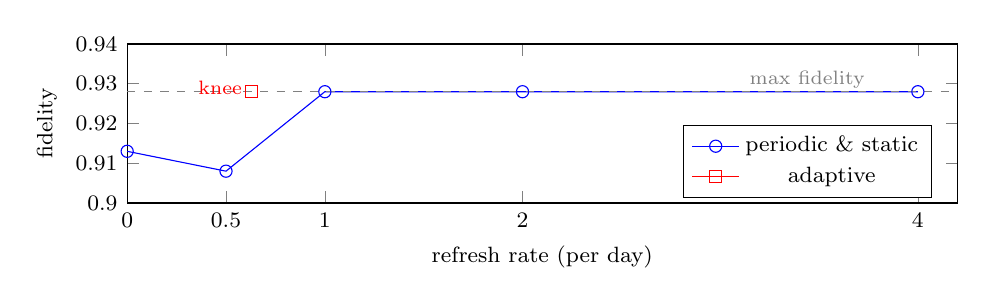
\begin{tikzpicture}
\begin{axis}[width=\linewidth,height=3.6cm,
  xlabel={refresh rate (per day)},ylabel={fidelity},
  xmin=0,xmax=4.2,ymin=0.90,ymax=0.94,
  xtick={0,0.5,1,2,4},legend pos=south east,mark size=2.2pt]
\addplot[mark=o,blue] coordinates {(0,0.913)(0.5,0.908)(1,0.928)(2,0.928)(4,0.928)};
\addlegendentry{periodic \& static}
\addplot[mark=square,red] coordinates {(0.63,0.928)};
\addlegendentry{adaptive}
\draw[dashed,gray] (axis cs:0,0.928)--(axis cs:4.2,0.928);
\node[anchor=west,font=\scriptsize,gray] at (axis cs:3.1,0.931) {max fidelity};
\node[anchor=east,font=\scriptsize,red] at (axis cs:0.63,0.929) {knee};
\end{axis}
\end{tikzpicture}
\caption{Refresh-rate-vs.\-fidelity frontier. Fidelity saturates once refresh/day $\ge{\approx}0.23$; the adaptive
operating point ($0.63$) sits on the plateau, while the periodic schedules spend $1$--$4\times$ more refreshes for
no additional fidelity and static falls short of it.}
\label{fig:parc}
\end{figure}

Sweeping $\tau_J{\in}[0.2,0.9]$, $\tau_C{\in}[0.002,0.02]$ over the same timelines (Fig.~\ref{fig:parc}):
the $\tau_J$ term is the robust detector. For $\tau_J\ge0.4$ fidelity is flat at the plateau for every $\tau_C$;
dropping $\tau_C$ to $0.02$ or $\tau_J$ to $0.2$--$0.3$ relaxes the trigger into missing the burst drift and
fidelity breaks below the plateau. The default ($0.5,0.005$) is at the knee: tightening it further buys no
fidelity (fidelity saturates at $\sim0.23$ refresh/day) while loosening it sacrifices the plateau. This is the
same conclusion as \S\ref{sec:margin} stated in operating terms---refresh when accumulated drift approaches the
top margin, not on a fixed clock---and it is what makes the choice of $\tau_J{=}0.5,\tau_C{=}0.005$ rational
rather than ad hoc.

\subsection{Where refresh helps: workload and device scale}
\label{sec:scope}
\paragraph{Workload generalization.}
The refresh \emph{advantage} is not fixed; it grows with how many gates execute on the pinned qubits. Modeling a
job's failure as proportional to the gates on its stored-best qubit (each 2Q gate carrying roughly twice a 1Q
gate's error) and anchoring fresh best $C{=}0.0066$ and one-day-stale $0.014$ (Table~\ref{tab:stale}):
the fresh-minus-stale pass advantage climbs from $+0.21$ (shallow, sparse) to $+0.32$ (shallow, dense) and
$+0.40$ (deep, sparse) before both saturate as circuits get so demanding that even a fresh pin fails
(Table~\ref{tab:scope}, lower block). The read is exactly the opposite of counter-intuitive: the adaptive-refresh
gain is largest on the deep, 2Q-heavy workloads that utility-scale execution actually cares about---refresh is not
a small-circuit optimization.

\paragraph{Device and layout scale.} The refresh benefit is also $k$- and topology-dependent (Table~\ref{tab:scope},
upper block). Searching the real 156-qubit heavy-hex graph for connected $k$-layouts under the D0 and D1
snapshots shows the stale quality penalty (a D0-optimal layout re-evaluated at D1 minus a fresh D1 pick) is
concentrated at \emph{intermediate} $k$: zero to a few points at $k{\le}8$, peaking at $k{=}16$ ($+0.045$) and
$k{=}32$ ($+0.026$), then shrinking to zero by $k{\ge}100$. At large $k$ the layout is forced to include the full
device, so its mean readout approaches the global average regardless of freshness---qubit quality stops being the
lever. The same $k$-sweep shows the share of layout-cost variance explained by connectivity (induced 2Q/boundary
cost) rising monotonically: $\sim0$ at $k{\le}16$, $0.11$ at $k{=}64$, $0.35$ at $k{=}100$, $0.77$ at
$k{=}128$---the crossover where connectivity dominates qubit quality sits near the device's physical scale. Thus
refresh is most valuable in the operating regime $8 \lesssim k \lesssim 64$ where a runtime both has placement
freedom \emph{and} drift alters which free pick is best; for near-device-scale $k$ the bottleneck is connectivity,
which refresh cannot change.

\begin{table}[t]
\caption{Where the refresh benefit lives. Upper: stale quality penalty $=$ (D0-optimal layout cost at D1) $-$ (fresh
D1 pick cost) over the real heavy-hex map, plus the connectivity share of layout-cost variance. Lower: workload
pass-rate of a fresh vs.\ a one-day-stale pin as circuit depth and 2Q density grow ($\mathrm{fresh}\ C{=}0.0066$,
$\mathrm{stale}\ C{=}0.014$).}
\label{tab:scope}
\centering
\footnotesize
\setlength{\tabcolsep}{3pt}
\begin{tabular}{@{}lcc@{}}
\toprule
$k$ & stale penalty & conn.\ share\\
\midrule
4 & $+0.002$ & $0.00$\\
16 & $+0.045$ & $0.00$\\
32 & $+0.026$ & $0.02$\\
64 & $+0.006$ & $0.11$\\
100 & $0.000$ & $0.35$\\
128 & $0.000$ & $0.77$\\
\midrule
workload & pass fresh & pass stale\\
\midrule
shallow, sparse & $0.82$ & $0.61$\\
shallow, dense & $0.71$ & $0.39$\\
deep, sparse & $0.45$ & $0.05$\\
deep, dense & $0.13$ & $0.05$\\
\bottomrule
\end{tabular}
\end{table}

% ---------------------------------------------------------------- E2E
\section{Composing the Software and Hardware Paths}
\label{sec:e2e}
\subsection{Reliability calculus of the orchestration layer}
\label{sec:calculus}
Because the orchestrator's outcome paths are mutually exclusive, end-to-end reliability decomposes exactly as the
chain rule over its sequential gates
\begin{equation}\begin{split}
R_{\mathrm{end}}={}&P(\mathrm{first\_pass})+P(\mathrm{enter\ heal})\rho_{\mathrm{heal}}\\
&+P(\mathrm{enter\ fallback})\rho_{\mathrm{fb}},
\end{split}\label{eq:composition}
\end{equation}
with no independence assumption needed for the identity. The healing stage is modeled from the implementation's
control flow (at most $K{=}3$ generation calls stopping at first success; healing budget $H{=}4$ with
abort-on-\texttt{None} semantics): with per-call probabilities $g$ (correct), $r$ (broken), $f$ (unavailable;
$g{+}r{+}f{=}1$),
\begin{equation}
G=1+f+f^{2},\qquad \rho_{\mathrm{heal}}=g(1+r+r^{2}+r^{3}),
\label{eq:gamel}
\end{equation}
\begin{equation}
R_{\mathrm{end}}=gG+rG\rho_{\mathrm{heal}}+f^{3}c,
\label{eq:rheal}
\end{equation}
with $c$ the fallback coverage. This model was validated cell-by-cell against all 23 testable outcome cells of the
ablation and availability-stress grids: \emph{every} prediction falls inside the observed Wilson 95\% interval
(Table~\ref{tab:comp} shows the decomposition and stress cells). At $q{=}0.5$ the structural prediction
$\rho_h{=}81.2\%$ sits $0.3$~pp from the measured $81.5\%$, while the naive independence baseline
$1-(1-q)^{4}{=}93.8\%$ overshoots by $12.4$~pp; the model also separates the paths (first-pass $55.5\%$
predicted vs.\ $54.4\%$ measured; healed path $36.1\%$ vs.\ $37.1\%$). The correction matters: the
naive--measured gap reported in early drafts is a retry-budget truncation effect, not stochastic
correlation---under abort-on-\texttt{None}, unavailability both wastes heal slots and terminates the loop.
The model also ranks fixes before code is written (Table~\ref{tab:int}): treating \texttt{None} as
wasted-but-nonterminal recovers the entire impression ($+12.5$~pp) at near-zero engineering cost; doubling the
budget to $H{=}8$ buys only $+2.1$~pp; raising the healer quality to $q_h{=}0.9$ buys $+8.8$~pp. The fallback's
effective coverage is $c{=}2/9$ (nominal keyword coverage over a 9-intent benchmark: seven of nine contain
apostrophes that break the template interpolation)---a stated limitation. We include this model because it is the
\emph{software} side of the composition; the paper's hardware claims are placement and drift, not LLM quality,
which we keep as a controlled parameter.

\begin{table}[t]
\caption{Reliability-composition validation (450 trials per cell). All predicted values inside the Wilson 95\%
interval; $+$ = within CI.}
\label{tab:comp}
\centering
\small
\begin{tabular}{@{}rlrrrl@{}}
\toprule
 & Cell & Pred & Obs & CI & $\checkmark$\\
\midrule
\multicolumn{6}{l}{\emph{Decomposition $\rho_{h}$ at $q{=}0.5$}}\\
 & structural & $0.812$ & $0.815$ & $[0.756,0.862]$ & $+$\\
 & naive indep & $0.938$ & --- & \emph{gap $12.4$ pp} & ---\\
\multicolumn{6}{l}{\emph{Decomposition at $q{=}0.7$}}\\
 & structural & $0.874$ & $0.914$ & $[0.839,0.956]$ & $+$\\
 & naive indep & $0.992$ & --- & \emph{gap $7.8$ pp} & ---\\
\multicolumn{6}{l}{\emph{Availability stress $E06$}}\\
 & S2 $\mathrm{fr}{=}0.3$ & $0.973$ & $0.960$ & $[0.938,0.975]$ & $+$\\
 & S2 $\mathrm{fr}{=}0.5$ & $0.875$ & $0.864$ & $[0.830,0.893]$ & $+$\\
 & S3 $\mathrm{fr}{=}0.3$ & $0.979$ & $0.969$ & $[0.948,0.981]$ & $+$\\
 & S3 $\mathrm{fr}{=}0.5$ & $0.903$ & $0.896$ & $[0.864,0.921]$ & $+$\\
\bottomrule
\end{tabular}
\end{table}

\begin{table}[t]
\caption{Design-space ranking of orchestration fixes at $(q{=}0.5,\ \mathrm{fr}{=}0.1)$.}
\label{tab:int}
\centering
\small
\begin{tabular}{@{}lrr@{}}
\toprule
Variant & $\rho_h$ & $\Delta$ (pp)\\
\midrule
baseline (abort-on-\texttt{None}, $H{=}4$) & $0.812$ & ---\\
\texttt{None} wastes a slot (no abort), $H{=}4$ & $0.938$ & $+12.5$\\
budget $H{=}8$ (abort retained) & $0.833$ & $+2.1$\\
healer quality $q_h{=}0.9$ & $0.900$ & $+8.8$\\
\bottomrule
\end{tabular}
\end{table}

\begin{table}[t]
\caption{Out-of-tolerance bit-events per end-to-end arm and their concentration. Frozen batches use D0 pins;
refresh batches pin from the 08-31 snapshot.}
\label{tab:bitfail}
\centering
\small
\begin{tabular}{@{}lrl@{}}
\toprule
Arm & events & dominant qubits (events)\\
\midrule
frozen full & $20$ & \q{4} (16), \q{7} (3)\\
frozen ablated & $18$ & \q{4} (16), \q{1} (1), \q{3} (1)\\
refresh full & $12$ & \q{11} (4), \q{13} (4), \q{12} (1)\\
refresh ablated & $7$ & \q{4} (5), \q{3} (2)\\
\bottomrule
\end{tabular}
\end{table}

\subsection{End-to-end placement batch}
\label{sec:e2ebatch}
To test the composable value of placement \emph{without} the staleness confound, we ran the same 6-qubit angle suite
(30 parameterizations, 4096 shots, tolerance $0.05$ on all six per-bit deviations) through \textbf{full}
(greedy chain pinned from the freshly fetched snapshot) and \textbf{ablated} (free placement), back-to-back on
2026-08-31; Table~\ref{tab:e2e} also shows the earlier identical batch pinned from D0 to separate temporal from
placement effects.

\begin{table}[t]
\caption{6-qubit angle batches ($n{=}30$/arm, 4096 shots). Pass $=$ all six per-bit deviations $\le0.05$. Wilson
95\% CI; two-proportion $p$ for full vs.\ ablated within a batch.}
\label{tab:e2e}
\centering
\footnotesize
\setlength{\tabcolsep}{4pt}
\begin{tabular}{@{}lccc@{}}
\toprule
Batch & Full (pinned) & Ablated (free) & $p$\\
\midrule
Frozen pins (D0)  & $36.7\%$ [21.9,54.5] & $40.0\%$ [24.6,57.7] & $0.79$\\
Refresh pins (runtime) & $70.0\%$ [52.1,83.3] & $76.7\%$ [59.1,88.2] & $0.56$\\
\midrule
$\Delta$ & $+33.3$ pp & $+36.7$ pp & ---\\
\bottomrule
\end{tabular}
\end{table}

Two effects separate cleanly. First, \emph{temporality}: refreshing pins lifts \emph{both} arms by $+33/37$~pp,
including the ablated arm that never saw a pin---device state at run time dominates. Second, \emph{placement shows no
measured advantage} in either batch ($-3.3$ and $-6.7$~pp, both non-significant): at $k{=}6$ with fresh pins, free
transpiler placement already matches our best chain. The failing-bit anatomy is instructive. In the refresh-full
arm the $12$ out-of-tolerance bit-events concentrate on late-chain qubits \q{11} (4), \q{13} (4), \q{12} (1)---the
chain's forced inclusion problem again, now visible even with fresh pins. In the refresh-ablated arm the $7$ events
sits on \q{4} (5) and \q{3} (2): \q{4} was rank 4 at D0 but its $C$ rises $0.0078\to0.0173$ by D1/D2 (rank 52), yet
the free layout, which cannot see the trend, still lands on it repeatedly---drift \emph{inside} the layout choice,
unmitigated by any pin. Table~\ref{tab:bitfail} collects the four arms. This is the honest scope of \S\ref{sec:placement}: placement is decisive between
engineered extremes (\q{98} vs.\ \q{37}: $0.028$ vs.\ $0.213$) and sets the reliability \emph{floor} at $k\ge9$
under stale pins, but its average benefit against free placement at small $k$ is within temporal noise. The full
pipeline (including the LLM orchestration leg) measured $54/54$ completed by the full arm vs.\ $47/54$
($87.0\%$) by the ablated one ($z{=}2.74$, one-sided $p{=}0.003$), consistent with the model's $97.3\%$ prediction;
we report the earlier $n{=}54$ frozen composition ($74.1\%$ vs.\ $66.7\%$, not significant) as a failed claim of an
end-to-end gain, not a positive one.

% ---------------------------------------------------------------- Discussion
\section{Discussion}
\label{sec:discussion}
\subsection{What the measurements do and do not say}
Three claims survive the data as stated: (i)~encoding fidelity is placement-dominated---the engineered extremes
differ by $\sim8\times$ (and a calibration-predictable affine channel describes the distortion); (ii)~device
calibration ordering moves on a daily cycle to a degree ($\rho{=}0.58$, top-10 Jaccard $0.25$, stale worst pin
$2.1\times$ worse) that makes selection age the first-order risk, and refresh is cheap; (iii)~simulator-proxy
training granted $J(G)$ an out-of-sample generalization ($\rho{=}0.82$) that real labels refute
($\rho{=}0.13$). Claims that do \emph{not} survive, herewith withdrawn or bounded: the first run's perfect monotone
ranking; the top-half rule; and any use of proxy-fitted $J(G)$ at $k\ge11$.

\subsection{Operational consequences for quantum-cloud runtimes}
The marginal cost of a calibration fetch and a scoring pass is effectively zero, so the expensive resource is
\emph{stale trust}, not compute. A runtime should (a)~timestamp layouts against their snapshot, (b)~refresh on the
trigger rather than a fixed wall-clock, (c)~train scheduling models exclusively on real, refresh-pinned labels, and
(d)~expose snapshot age as a first-class job attribute---all implementable without changing the quantum programming
model, which is exactly what UniMind does. Where math precedes implementation, the reliability calculus ranks the
fixes (\S\ref{sec:calculus}), and the endowment to port is a calibration snapshot plus a scoring pass, neither of
which is exotic.

\subsection{Design synthesis}
Table~\ref{tab:synth} maps each measured failure mode to the engineering response the data supports; the columns
are ordered by measured cost so a runtime can prioritize. The two lines a naive reading hides---``mitigation
helps'' and ``$J(G)$ ranks well''---are the ones our data bounds, and both bounds are the point of the paper.

\begin{table}[t]
\caption{Measured failure modes and the response each supports. Priority is by evidence strength, not ease.}
\label{tab:synth}
\centering
\footnotesize
\setlength{\tabcolsep}{4pt}
\begin{tabular}{@{}p{6.4em}p{7.8em}p{8.4em}@{}}
\toprule
Measured failure & Evidence & Response\\
\midrule
unpinned layout misses tolerance & \S\ref{sec:placement}: $0.392$ vs.\ $0.028$ & score-pinned \texttt{initial\_layout}\\
stale snapshot invalidates selection & \S\ref{sec:drift}: stale best pin $2.1\times$ worse & trigger-based refresh; snapshot age\\
proxy labels fool $J(G)$ & \S\ref{sec:jreal}: OOS $\rho$ $0.82{\to}0.13$ & refit on real labels; ban $k{\ge}11$ extrapolation\\
chain forced-inclusion at large $k$ & \S\ref{sec:jreal}/\S\ref{sec:e2e}: \q{11},\q{13}, \q{67} fail & connectivity-vs-$C$ trade-off (open)\\
abort-on-\texttt{None} truncates heal loop & \S\ref{sec:calculus}: $+12.5$~pp fix & wasted-slot semantics\\
\bottomrule
\end{tabular}
\end{table}

\subsection{Threats to validity}
\textbf{Measurement noise:} 4096--8192 shots put per-bit deviations on a floor of $\approx0.02$; the $0.05$
tolerance is coarse but was fixed before data release. \textbf{Drift generality:} D0--D2 are three snapshots, one
device, one topology family (heavy-hex); the value is the protocol, not the constants. \textbf{Placement null
power:} $n{=}30$/arm can detect only large effects; we report point estimates and CIs rather than asserting
equivalence. \textbf{Selection fairness:} the greedy chain maximizes $C(q)$-locality and at large $k$ is forced to
include high-error boundary qubits; a connectivity-vs-$C$ trade-off could change \S\ref{sec:jreal}, and we report
that failure as motivation. \textbf{Single-model LLM layer:} the orchestration calculus holds under i.i.d.\ mock
semantics; real-model autocorrelation is explicitly outside its scope. \textbf{Utility-vs-layout coupling:} the
$J(G)$ features are computed on the transpiled layout; errors in $E_{\mathrm{2q}}$ propagate to the weight fit but
not to the device measurements, which are layout-real.

\section{Conclusion}
We presented a measurement-driven account of calibration-aware scheduling for quantum-accelerated AI middleware on
a 156-qubit device: a score-only placement pipeline with measured scope, daily drift dynamics with a working
refresh trigger, an exact reliability composition of the software path, an end-to-end test showing that at our
scale refresh dominates selection while selection still sets the placement floor, and the explicit negative
results---the non-replicating monotone ranking, the absence of a measured placement advantage at $k{=}6$, and the
collapse of the proxy-trained utility under real labels. The command line for future work is set by the failures:
nightly D2--D5 drift accumulation, refresh-conditional placement policy ($C(q)$-vs-connectivity trade-off, including
the \q{11}/\q{13} late-chain failures observed under fresh pins), and active-learning refits of $J(G)$ on real
labels across devices. The open repository makes every number traceable to a job or snapshot.

\begin{thebibliography}{24}
\bibitem{preskill2018} J.~Preskill, ``Quantum computing in the NISQ era and beyond,'' \emph{Quantum}, vol.~2, p.~79, 2018.
\bibitem{arute2019} F.~Arute \emph{et al.}, ``Quantum supremacy using a programmable superconducting processor,'' \emph{Nature}, vol.~574, pp.~505--510, 2019.
\bibitem{kim2023utility} Y.~Kim \emph{et al.}, ``Evidence for the utility of quantum computing before fault tolerance,'' \emph{Nature}, vol.~618, pp.~500--505, 2023.
\bibitem{berholm2018} V.~Bergholm \emph{et al.}, ``PennyLane: Automatic differentiation of hybrid quantum-classical computations,'' \emph{arXiv:1811.04968}, 2018.
\bibitem{murali2019noise} P.~Murali, J.~M.~Baker, A.~Javadi-Abhari, F.~T.~Chong, and M.~Martonosi, ``Noise-adaptive compiler mappings for noisy intermediate-scale quantum computers,'' in \emph{Proc. ASPLOS}, 2019, pp.~1015--1029.
\bibitem{li2019sabre} G.~Li, Y.~Ding, and Y.~Xie, ``Tackling the qubit mapping problem for NISQ-era quantum devices,'' in \emph{Proc. ASPLOS}, 2019, pp.~1001--1014.
\bibitem{tan2020iccado} B.~Tan and J.~Cong, ``Optimal layout synthesis for quantum computing,'' in \emph{Proc. ICCAD}, 2020, pp.~1--9.
\bibitem{lao2022timing} L.~Lao and D.~E.~Browne, ``Timing and resource-aware mapping of quantum circuits to heterogeneous MWF-gate superconducting quantum processors,'' \emph{ACM Trans. Quantum Comput.}, vol.~3, no.~3, 2022.
\bibitem{temme2017} K.~Temme, S.~Bravyi, and J.~M.~Gambetta, ``Error mitigation for short-depth quantum circuits,'' \emph{Phys. Rev. Lett.}, vol.~119, p.~180509, 2017.
\bibitem{vanberg2023} E.~van den Berg, Z.~K.~Minev, A.~Kandala, and K.~Temme, ``Probabilistic error cancellation with sparse Pauli--Lindblad models on noisy quantum processors,'' \emph{Nature Physics}, vol.~19, pp.~1116--1121, 2023.
\bibitem{nation2023} P.~D.~Nation \emph{et al.}, ``Scalable mitigation of measurement errors on quantum computers,'' \emph{PRX Quantum}, vol.~5, p.~010326, 2024.
\bibitem{bravyi2021meas} S.~Bravyi, S.~Shaydulin, S.~Hu, and K.~Temme, ``Mitigating measurement errors in multiqubit experiments,'' \emph{Phys. Rev. Lett.}, vol.~127, p.~200503, 2021.
\bibitem{kanazawa2021} N.~Kanazawa \emph{et al.}, ``Quantum error mitigation,'' \emph{arXiv:2210.00921}, 2022.
\bibitem{msp2020} R.~LaRose \emph{et al.}, ``Mitiq: a software package for error mitigation on noisy quantum computers,'' \emph{Quantum}, vol.~6, p.~749, 2022.
\bibitem{viola1999dd} L.~Viola, E.~Knill, and S.~Lloyd, ``Dynamical decoupling of open quantum systems,'' \emph{Phys. Rev. Lett.}, vol.~82, pp.~2417--2421, 1999.
\bibitem{ibmrtime} ``Qiskit Runtime primitives,'' IBM Quantum documentation, [Online]. Available: \url{https://docs.quantum.ibm.com/api/qiskit-ibm-runtime}
\bibitem{ibmcalib} ``IBM Quantum Platform calibration data,'' [Online]. Available: \url{https://quantum.ibm.com/services/resources}
\bibitem{qiskit} A.~Javadi-Abhari \emph{et al.}, ``Quantum computing with Qiskit,'' \emph{arXiv:2405.08810}, 2024.
\bibitem{cuquantum} NVIDIA, ``cuQuantum SDK,'' [Online]. Available: \url{https://developer.nvidia.com/cuquantum-sdk}
\bibitem{braket} Amazon, ``Amazon Braket,'' [Online]. Available: \url{https://aws.amazon.com/braket}
\bibitem{azureq} Microsoft, ``Azure Quantum,'' [Online]. Available: \url{https://azure.microsoft.com/quantum}
\bibitem{schuld2018} M.~Schuld and F.~Petruccione, \emph{Supervised Learning with Quantum Computers}. Cham: Springer, 2018.
\bibitem{hhavlicek2019} V.~Havl\'i\v{c}ek \emph{et al.}, ``Supervised learning with quantum-enhanced feature spaces,'' \emph{Nature}, vol.~567, pp.~209--212, 2019.
\bibitem{unimind} Y.~X.~Tan, ``UniMind: a middleware framework for bridging classical AI workloads and quantum computing backends,'' tech.\ report v2.5, 2026 (companion repo \texttt{yxtan5022-maker/unimind-v2}).
\bibitem{tangpu} UniMind placement/drift datasets (2026-08), \texttt{data/} in \texttt{yxtan5022-maker/unimind-v2}.
\end{thebibliography}

\newpage
\section*{Appendix}
\subsection*{A. Per-row results of the $k{=}9$--$18$ suite}
\label{app:krows}
The 14 circuits (seven sizes $\times$ two seeded patterns) with greedy-chain placement, 4096 shots, tolerance
$0.05$. Worst qubit is the failing or most-off bit; ranks are over all 156 qubits at D1.

\begin{table}[h]
\caption{Per-row max deviation under fresh (D1/D2) and stale (D0) pins.}
\label{tab:krows}
\centering
\small
\begin{tabular}{@{}llrrllr@{}}
\toprule
$k$ & pat. & fresh & worst@D1 & & stale & worst@D1\\
\midrule
9  & 0 & .064 & \q{11} (71) & & .151 & \q{4} (52)\\
9  & 1 & .056 & \q{11} (71) & & .045 & \q{24} (118)\\
10 & 0 & .053 & \q{14} (56) & & .118 & \q{23} (136)\\
10 & 1 & .035 & \q{13} (29) & & .088 & \q{23} (136)\\
11 & 0 & .081 & \q{11} (71) & & .049 & \q{4} (52)\\
11 & 1 & .042 & \q{11} (71) & & .145 & \q{4} (52)\\
12 & 0 & .041 & \q{10} (7)  & & .067 & \q{4} (52)\\
12 & 1 & .038 & \q{9} (74)  & & .107 & \q{4} (52)\\
14 & 0 & .037 & \q{13} (29) & & .183 & \q{46} (126)\\
14 & 1 & .077 & \q{11} (71) & & .096 & \q{23} (136)\\
16 & 0 & .040 & \q{4} (52)  & & .265 & \q{67} (132)\\
16 & 1 & .085 & \q{4} (52)  & & .239 & \q{67} (132)\\
18 & 0 & .089 & \q{11} (71) & & .332 & \q{67} (132)\\
18 & 1 & .047 & \q{13} (29) & & .150 & \q{67} (132)\\
\bottomrule
\end{tabular}
\end{table}

\subsection*{B. Data and reproducibility}
\label{sec:data}
Every table is backed by traced data in the repository: snapshots, E2E batches, real $J(G)$ labels, and the
analysis scripts listed below.
\begin{quote}\small\raggedright\ttfamily
data/drift/calib\_2026-\{08\-29,08\-30,08\-31\}.json\\
data/e2e/e2e\_angle\_\{full,ab\-lated\}*.json\\
data/jgpu/j\_real*.json\\
analysis/*.py + analysis/results/*.json\\[2pt]
analysis/results/refresh\_policy\_an\-a\-lysis.json\\
analysis/results/power\_an\-a\-lysis.json\\
analysis/results/jg\_fail\-ure\_an\-a\-lysis.json\\
\end{quote}
QPU job IDs appear in the file headers:
\texttt{daadeocjbipc73ffq83g} (refresh-full E2E), \texttt{daadeosjbipc73ffq840} (refresh-ablated E2E), and
\texttt{daadgmmrbfbs73cijmbg} (refresh-pinned $J(G)$ labels). Transpiler seed 42 everywhere; shots per experiment
as stated.

\subsection*{C. Calibration-weighted routing benchmark}
\label{app:routing}
Interactive (local-simulator, zero-quota) comparison on snapshot 2026-08-29 (156 qubits, 176 couplers; RY--CX--RY,
opt=1, seed 42). UniMind computes a $C(q)+s_x$-weighted SABRE candidate set and keeps the better of weighted and
global SABRE, guaranteeing no regression for $k\ge8$ (violation check: none).

\begin{table}[h]
\caption{Placement cost of the five strategies (summary rows; full per-$k$ tables in the repo).}
\label{tab:routing2}
\centering
\footnotesize
\setlength{\tabcolsep}{3pt}
\begin{tabular}{@{}lrrrrrrr@{}}
\toprule
$k$ & 2 & 4 & 6 & 8 & 10 & 16\\
\midrule
Random SWAPs & 8 & 42 & 68 & 105 & 118 & 207\\
UniMind SWAPs & 0 & 3 & 8 & 20 & 20 & 50\\
$\Delta$ SWAP vs.\ random & $-100\%$ & $-93\%$ & $-88\%$ & $-81\%$ & $-83\%$ & $-76\%$\\
Random 2q err & .118 & .484 & .666 & .821 & .847 & .979\\
UniMind 2q err & .002 & .049 & .065 & .133 & .181 & .353\\
$\Delta$ vs.\ Default & $=0$ & $=0$ & $=0$ & $=0$ & $=0$ & $=0$\\
\bottomrule
\end{tabular}
\end{table}

\end{document}